\documentclass{article}
\usepackage{graphicx} % Required for inserting images

\usepackage{amsmath}
\usepackage{amssymb}
\usepackage{bbm}
\usepackage{biblatex}
\usepackage{xcolor}
\usepackage{subcaption}
\addbibresource{ref.bib}

\newcommand{\E}{\mathbb{E}}
\newcommand{\R}{\mathbb{R}}
\newcommand{\abs}[1]{\left|#1\right|}
\newcommand{\var}[1]{\text{Var}\left(#1\right)}
\newcommand{\dd}[1]{\,\text{d}#1}

\title{Mathematical Statistics Final Project: Variable Kernel Density Estimation}
\author{Nick DeFilippis and Paco Rilloraza}
\date{12 December 2024}

\begin{document}

\maketitle

The fundamental question of statistics is the following: given observations $X_1, \dots, X_n$, from what probability measure did they arise? Often our candidate distributions arise from a family of measures $\mathcal{P}$ that can be parameterized by a parameter set $\Theta \subseteq \R^k$, i.e., for each $\theta \in \Theta$, there is a measure $\mathbb{P}_\theta \in \mathcal{P}$ \cite{jnw}. Assuming that $\theta \neq \theta'$ implies that $\mathbb{P}_\theta \neq \mathbb{P}_{\theta'}$, the question of finding the measure that explains our observations is equivalent to finding the optimal parameter. 

However, there are many cases in which $\mathcal{P}$ cannot be naturally parametrized. In this case, to find the explanatory $\mathbb{P} \in \mathcal{P}$, we must resort to the methods of nonparametric statistics. One such method is \textit{kernel density estimation} (KDE). KDE is a method for constructing an estimator $\hat{f}$ of a sufficiently smooth probability density $f$ from data. Such an estimator can be written as a sum of kernel functions centered at the data. Each of these kernel functions is a bump, and in most applications, the widths of these bumps are equal. In this setting, the figure of merit of the estimator is the \textit{mean-integrated square error} (MISE). In \cite{vkde}, Terrell and Scott study two proposals for KDEs with variable width, contrasting the MISEs of these variable KDEs with results from the fixed-width setting at varying numbers of samples $n$ and dimension $d$. 

{\color{blue} Paco: finish this once rest of write-up is done. Conclude: most of the results are negative.}

\section{Introduction and generalized kernels}
% 1. Introduction. Two types of VKDEs: h is a f'n of y or x. First promising for high dimensions, second for moderate sample sizes, but both bad

The standard form of a nonparametric kernel density estimator with a fixed bandwidth is
\begin{equation}\label{eq:fixed-width-kde}
    \hat{f}(\mathbf{y}) = \frac{1}{nh^d}\sum_{i=1}^nK\left(\frac{\mathbf{X}_i-\mathbf{y}}{h}\right)
\end{equation}

where $\mathbf{X}_i$ is an i.i.d random variable drawn from $\mathbf{P}_\theta$, and $K \in L^1(\R) \cap L^2(\R)$ is an order-$p$ kernel function, i.e., a unit mass function $K$ with $\lim_{z \to \infty} \abs{zK(z)} = 0$ and first nonzero moment being the $p$th moment, which is $\pm 1$ \cite{vkde}. Terrell and Scott introduce the idea of varying the size of the bandwidth

{\color{blue} motivate the two types of estimators a la the paragraph right before section 3 in the paper}

% 2. Generalized kernels. Multivariate density estimators that are continuous and Gateaux (directionally) differentiable can be written as an average of the Gateaux derivatives. Asymptotically, these become generalized KDEs. KDEs are (1) weights centered at y that specify how x_i influence estimate at y and (2) mixture of densities centered at x_i. VKDEs generalize these.
Noting that fixed-width KDEs receive the difference $\mathbf{X}_i-\mathbf{y}$ as an argument to $K$, the most broad generalization is an estimator of the form 
\begin{equation}\label{eq:gen-kde}
    \hat{f}(\mathbf{y}) = \frac{1}{n} \sum_{i=1}^n K_n(\mathbf{X}_i,\mathbf{y}) 
\end{equation}
for a suitable function $K_n$. To justify this form, the authors provide Theorem 1, which states that for any multivariate density estimator $\hat{f}$ that is sufficiently smooth, we can write 
\begin{equation}\label{eq:thm1}
    \hat{f}(\mathbf{y}) = \frac{1}{n} \sum_{i=1}^n K(\mathbf{X}_i,\mathbf{y},\hat{F}_n)
\end{equation}
where $K(\mathbf{X}_i,\mathbf{y},\hat{F}_n)$ is a particular directional derivative of $\hat{f}$ {\color{blue} (Paco: clarify)} that depends on the empirical cumulative distribution function (CDF) $\hat{F}_n$, i.e., it depends on all of the data $(\mathbf{X}_i)_{i=1}^n$. However, for large $n$, the Glivenko-Cantelli theorem \cite{jnw} says that $\hat{F}_n$ uniformly converges to the true CDF $F$, so in this limit, $K\mathbf{X}_i,\mathbf{y},\hat{F}_n)$ depends on $F$ and is thus independent of all of the data except for $\mathbf{X}_i$. Thus, equation \eqref{eq:thm1} can asymptotically be written as equation \eqref{eq:gen-kde}. 

\section{Univariate balloon estimators}
% 3. Balloon estimators have no AMISE improvement
Restricting to the one-dimensional setting, a univariate balloon estimator is a variable KDE of the form 
\begin{equation}\label{eq:balloon1}
    \hat{f}(y) = \frac{1}{nh(y)} \sum_{k=1}^n K\left(\frac{X_i-y}{h(y)}\right), 
\end{equation}
where $K$ is an order-$p$ univariate kernel. It is similar in form to a fixed-width KDE, except that the width $h$ depends on the observation point $y$. As in the fixed-width case, we have the asymptotic behavior
\begin{align}
    \var{\hat{f}(y)} &= O\left(\frac{1}{nh(y)}\right), \label{eq:ub-var} \\
    \left( \E \hat{f}(y) - f(y) \right)^2 &= O\left(h^p\right). \label{eq:ub-bias}
\end{align}
Recalling that the MISE is the integral of the sum of these, simple calculus shows that asymptotically the optimal bandwidth is $h \asymp n^{-1/(2p+1)}$, in which case the MISE is $O\left(n^{-2p/(2p+1)}\right)$. Fixed-width and balloon estimators thus have asymptotic MISEs that differ only by a constant factor which, for reference, is 
\begin{equation}\label{eq:ub-compare}
    \frac{\text{balloon asymptotic MISE}}{\text{fixed-width asymptotic MISE}} = \dfrac{\displaystyle\int f^{2p/(2p+1)} (f^{(p)})^{2/(2p+1)}}{\left[ \displaystyle\int (f^{(p)})^2 \right]^{1/(2p+1)}} \leq 1. 
\end{equation}
 However, a numerical experiment with Gaussian and Cauchy densities estimated with kernels at several orders demonstrates that this factor is commonly around 0.7 to 0.95. Thus in the univariate case, balloon estimators do not drastically improve the convergence rate of the MISE. To emphasize this point, the authors discuss a commonly used balloon estimator by Loftsgaarden and Quesenberry with $h(y)$ being the Euclidean distance between $y$ and the $k$th nearest datum. They show that the bias term contributes infinitely to the asymptotic MISE, yielding an improvement factor of zero, unless certain restrictive conditions on the density $f$ are met. For these reasons, the authors aptly conclude that in the univariate setting, balloon estimators are are ``mostly hot air.''

\section{Sample smoothing estimators}
% 4. Sample smoothing kernels have improved MISE for few samples, but no O(n^-8/9). Why? In the Gaussian data and uniform kernel case, the bias integral has some tail contributions yet unaccounted. There are different optimal bandwidths for n < 500 and n -> \infty. However a monotonicity condition in this result complicates analysis
Remaining in the one-dimensional setting, a sample smoothing estimator is a variable KDE of the form 
\begin{equation}\label{eq:ss1}
    \hat{f}(y) = \frac{1}{n} \sum_{k=1}^n \frac{1}{h(X_i)}K\left(\frac{X_i-y}{h(X_i)}\right), 
\end{equation}
with $K$ again an order-$p$ univariate kernel. Here, $h$ depends on the datum $X_i$. The authors show that while the asymptotic variance has the same form as equation \eqref{eq:ub-var}, the bias is 
\begin{equation}
    \left(\E \hat{f}(y) - f(y)\right)^2 \sim \left( \frac{1}{p!} \frac{\text{d}^p}{\text{d}y^p} \left(h(y)^pf(y)\right) \right)^2
\end{equation}

\section{Multivariate balloon estimators}
% 5. Multivariate balloon estimators can perform better at high dimensions

\section{Numerical experiment}

Finally, we perform a numerical experiment comparing balloon and sample smoothing estimators with a fixed-width kernel density estimator. We first generate $N$ samples from a standard $d$-dimensional multivariate Gaussian distribution.

Our control estimator is a fixed-bandwidth estimator using a Gaussian kernel. Specifically, we use
\begin{equation}
    K_\textup{fixed-gaussian}(\mathbf{x}) = (2\pi)^{-d/2}\exp\left(-\frac{\mathbf{x}^T\mathbf{x}}{2}\right)
\end{equation}.

We choose $h \propto n^{-1/(d+4)}$, as this choice leads to an optimal MISE \cite{jnw}. Then, our fixed-width estimate is found by equation \eqref{eq:fixed-width-kde} with $K_\textup{fixed-gaussian}$ as our kernel.

For our balloon and sample smoothing estimator, we use a uniform density on the unit $d$-sphere, specifically,
\begin{equation}
    K_{\textup{variable}}(\mathbf{x}) = \frac{\Gamma(d/2+1)}{\pi^{d/2}}\mathbbm{1}_{\vert\mathbf{x}\vert\leq1}(\mathbf{x})
\end{equation}

For simplicity, we choose $k \propto \sqrt{N}$ for the k-nearest neighbor component. Note that this still respects the asymptotic limit $k/n \rightarrow 0$ and $k\rightarrow \infty$. Our balloon estimate is found using \eqref{eq:balloon1} and our sample smoothing estimate using \eqref{eq:missing}.

Finally, we need to compute the MISE to compare our estimators. In higher dimensions, this becomes difficult if we use a direct numerical integration. Therefore, we estimate the MISE using a Monte-Carlo integration method. Figure \ref{fig:MISE} shows the MISE for dimensions $d=1$ through $d=6$.

\begin{figure}
\begin{subfigure}{.5\textwidth}
  \centering
  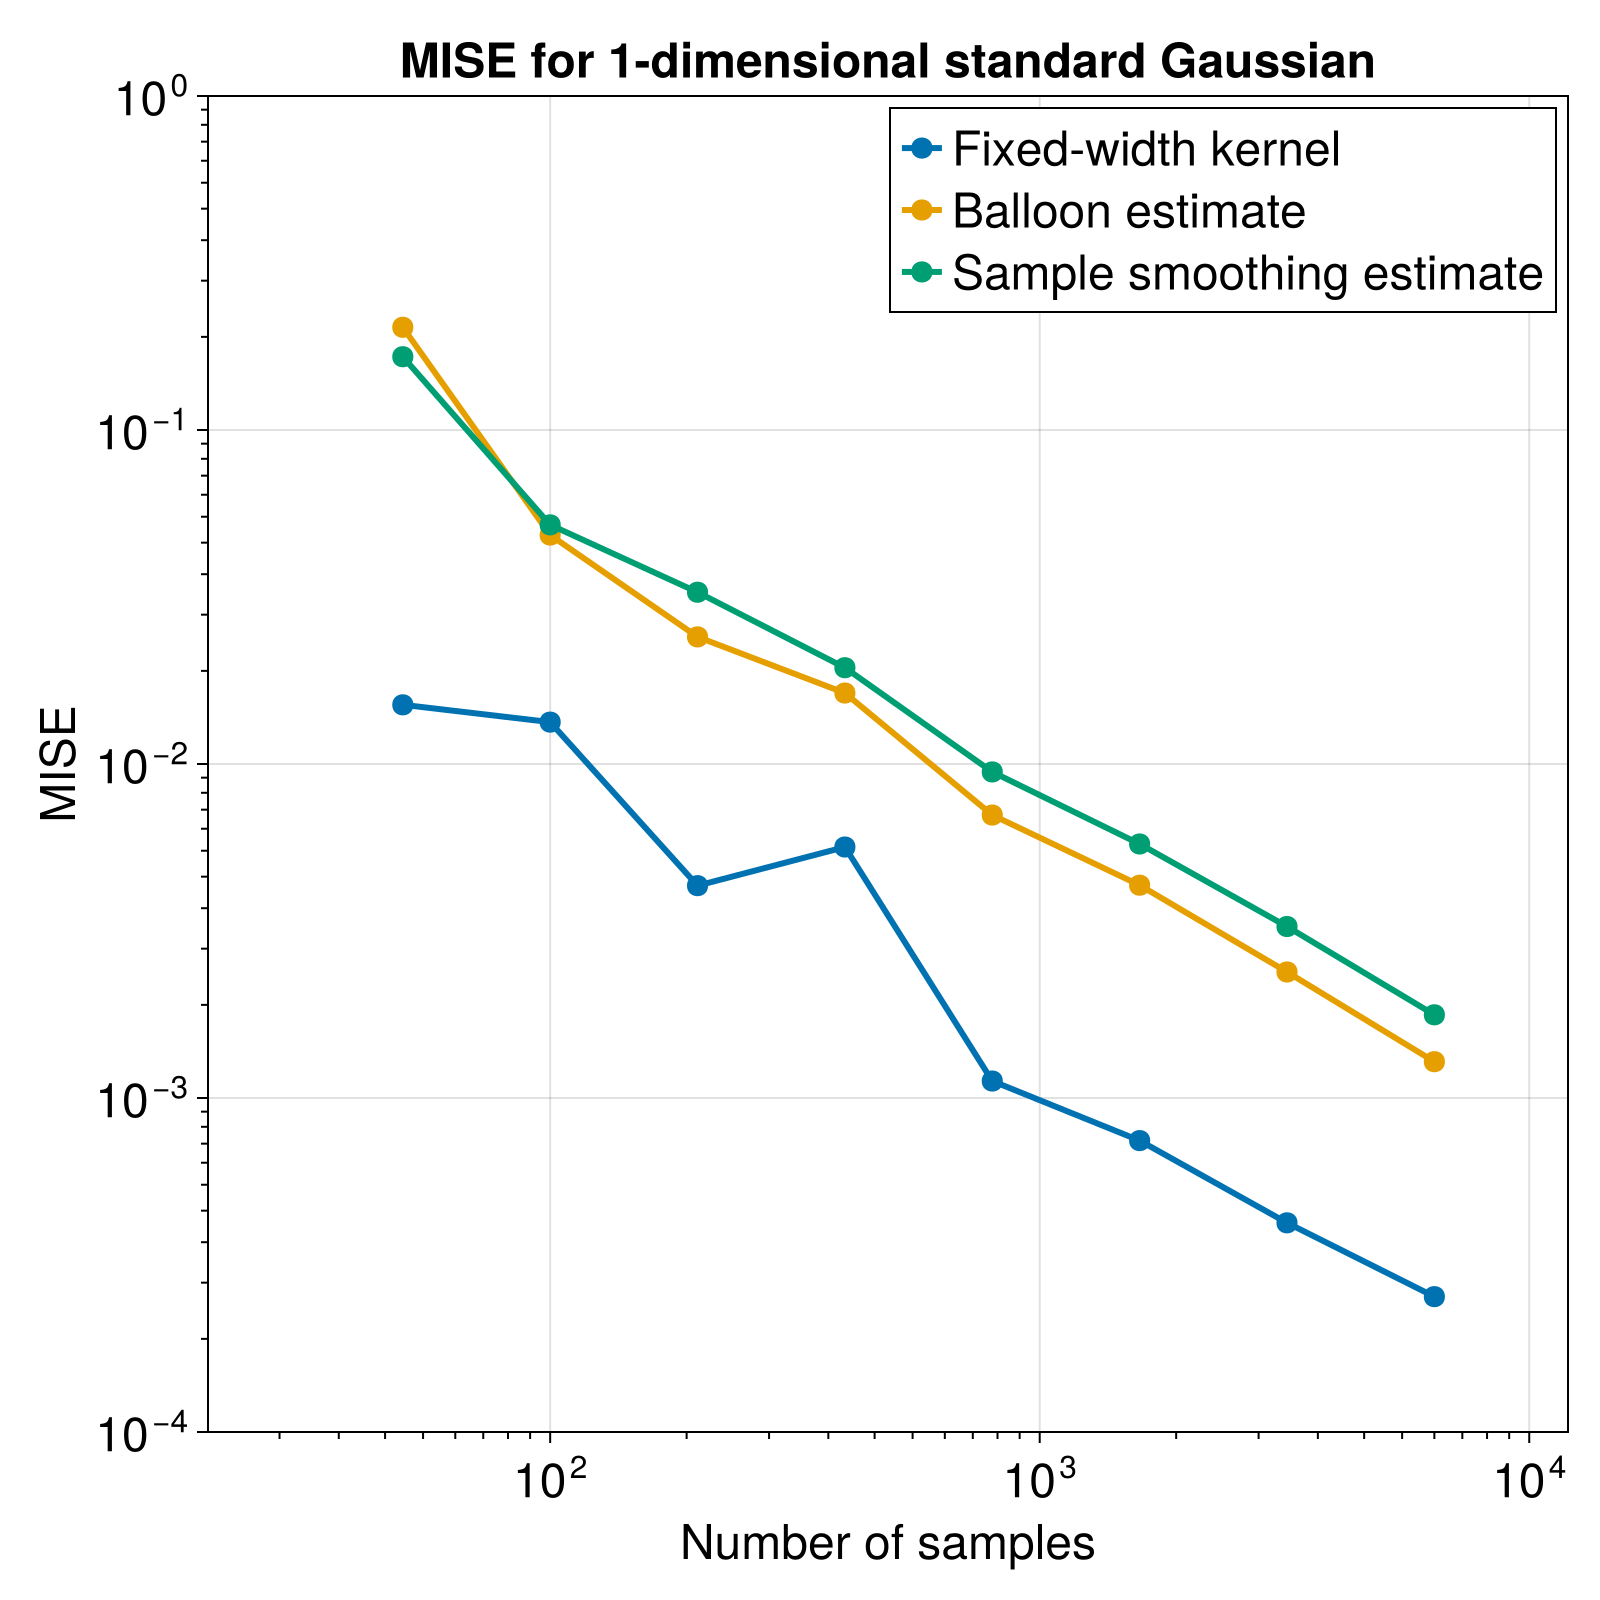
\includegraphics[width=.8\linewidth]{images/MISE_d=1.png}
  \caption{d=1}
  \label{fig:sfig1}
\end{subfigure}%
\begin{subfigure}{.5\textwidth}
  \centering
  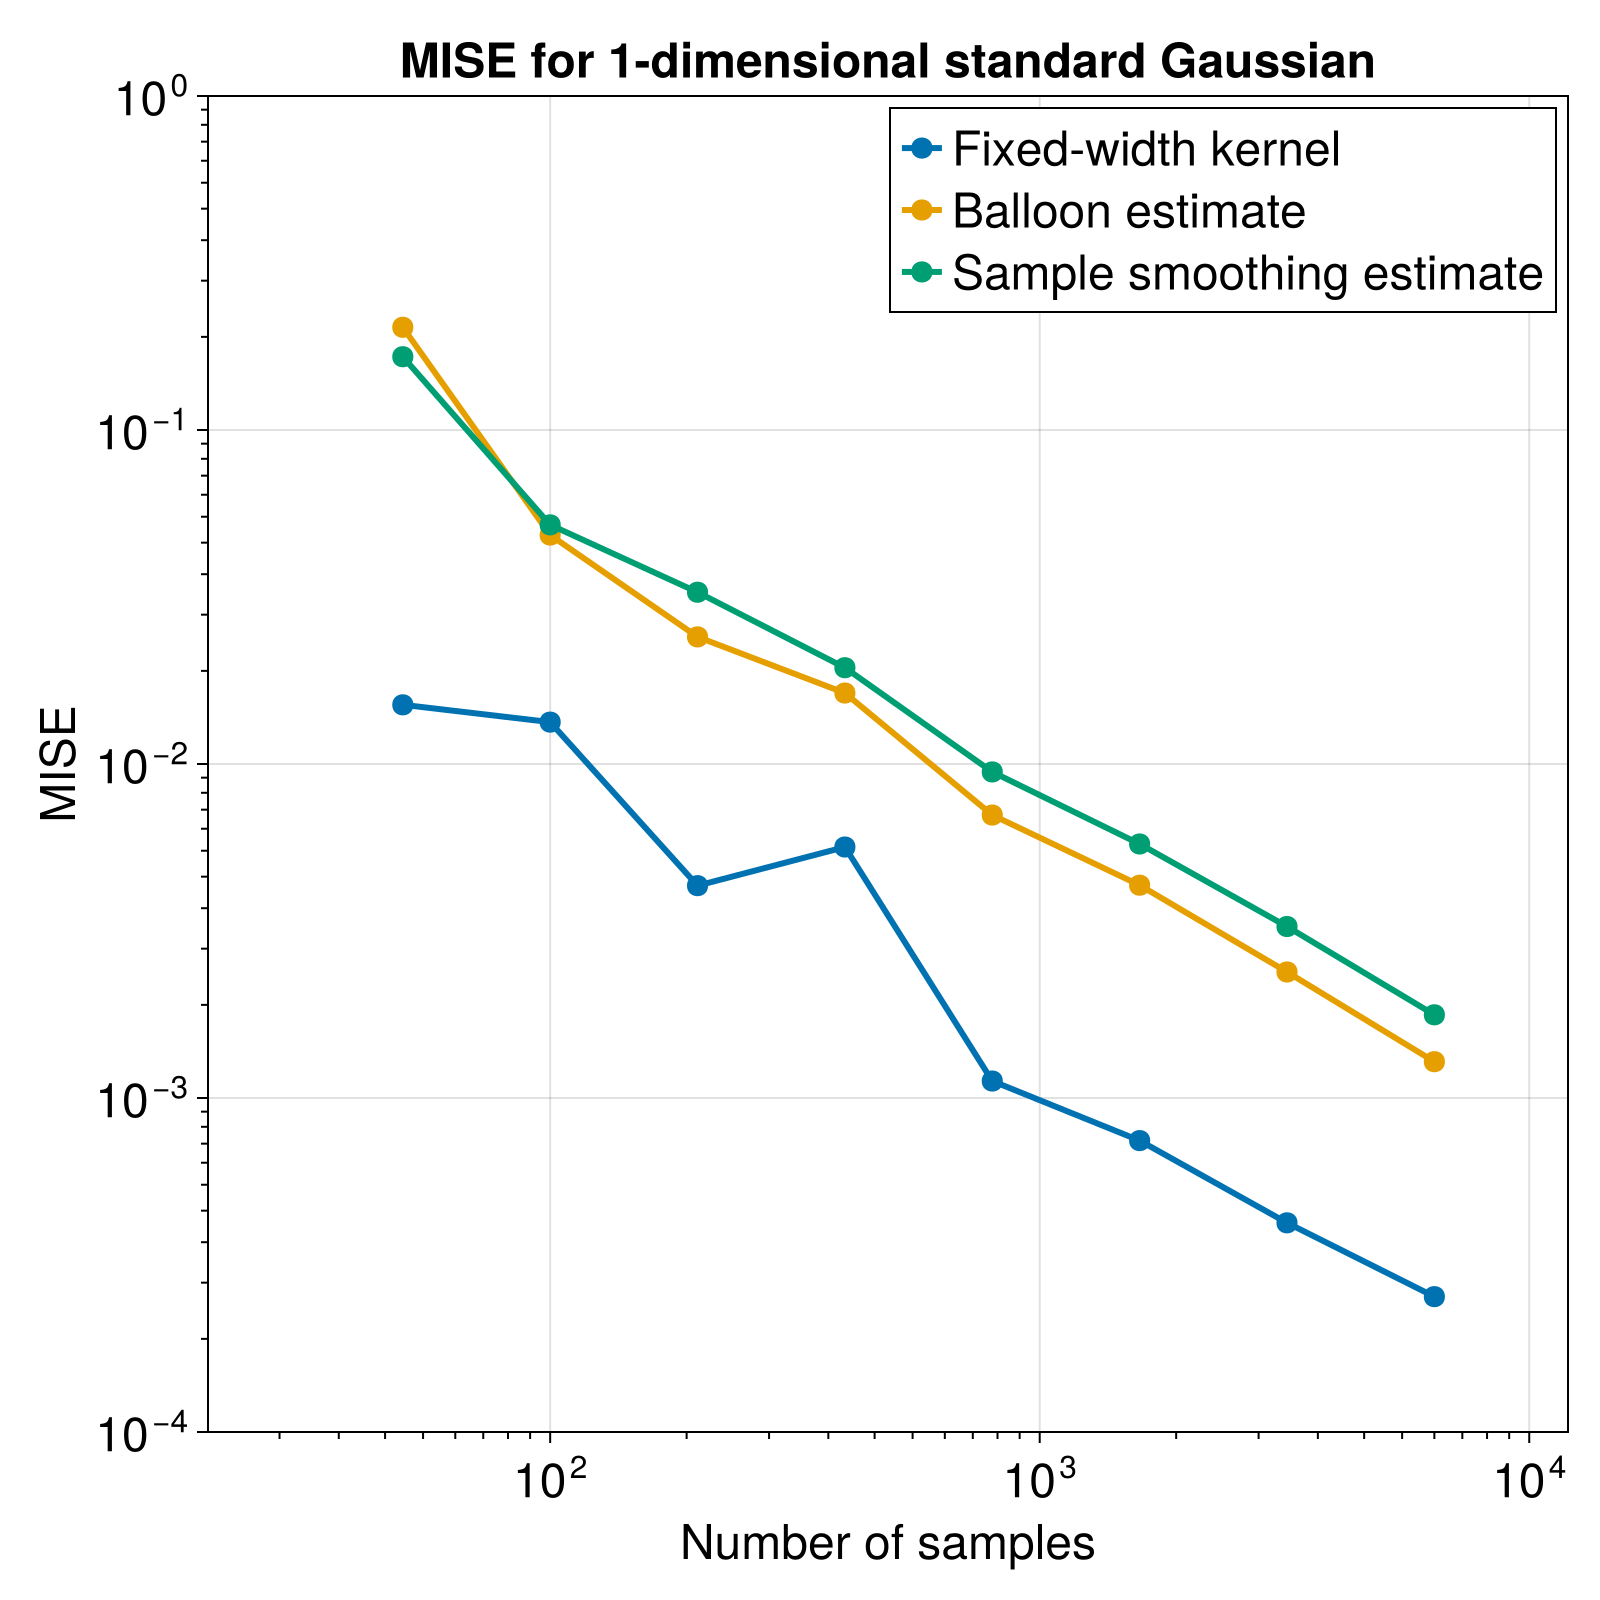
\includegraphics[width=.8\linewidth]{images/MISE_d=1.png}
  \caption{d=2}
  \label{fig:sfig2}
\end{subfigure}
\begin{subfigure}{.5\textwidth}
  \centering
  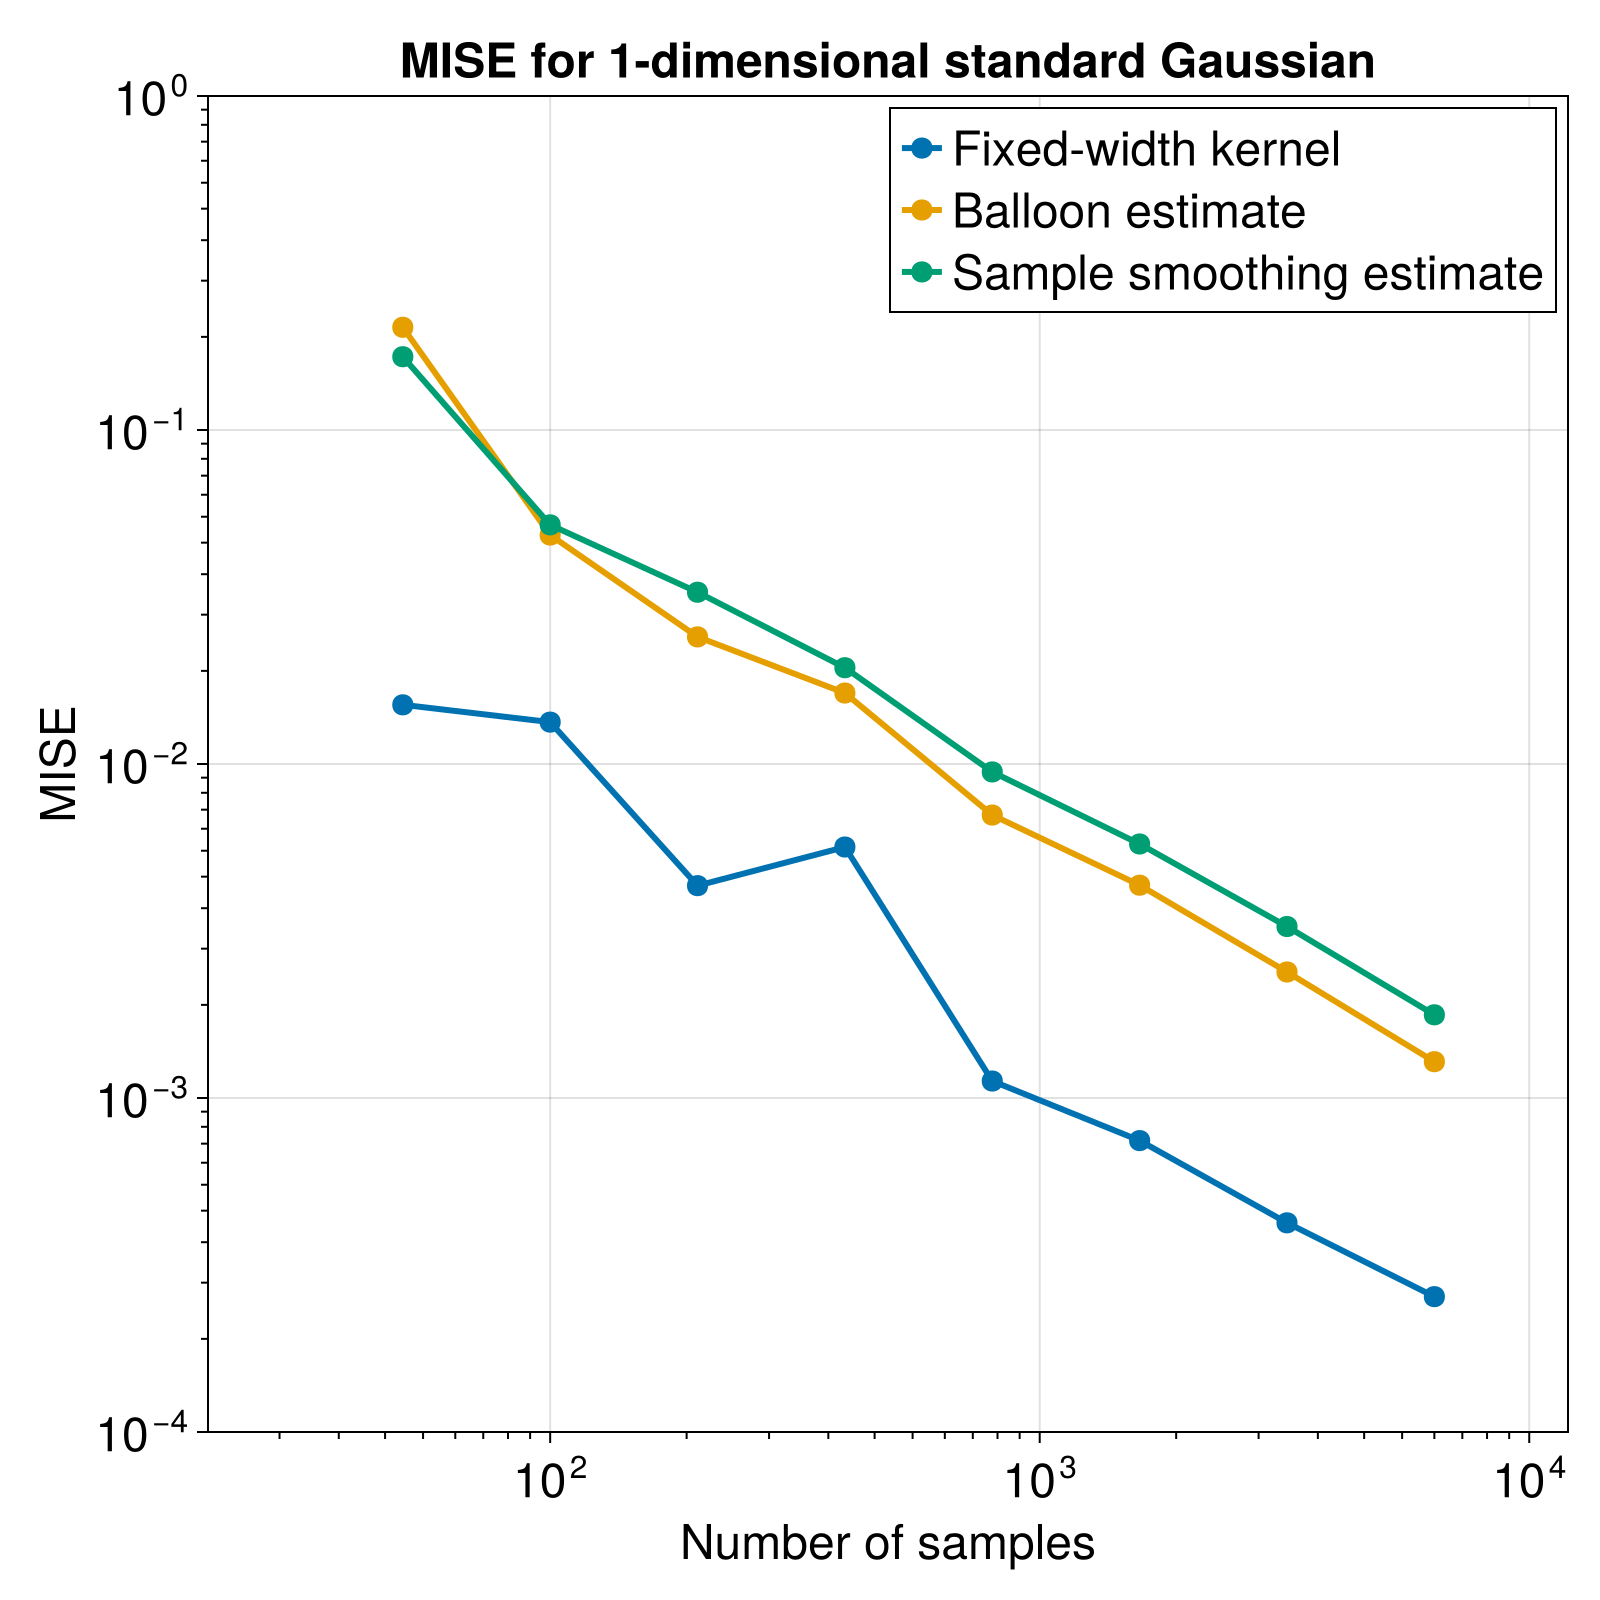
\includegraphics[width=.8\linewidth]{images/MISE_d=1.png}
  \caption{d=3}
  \label{fig:sfig1}
\end{subfigure}%
\begin{subfigure}{.5\textwidth}
  \centering
  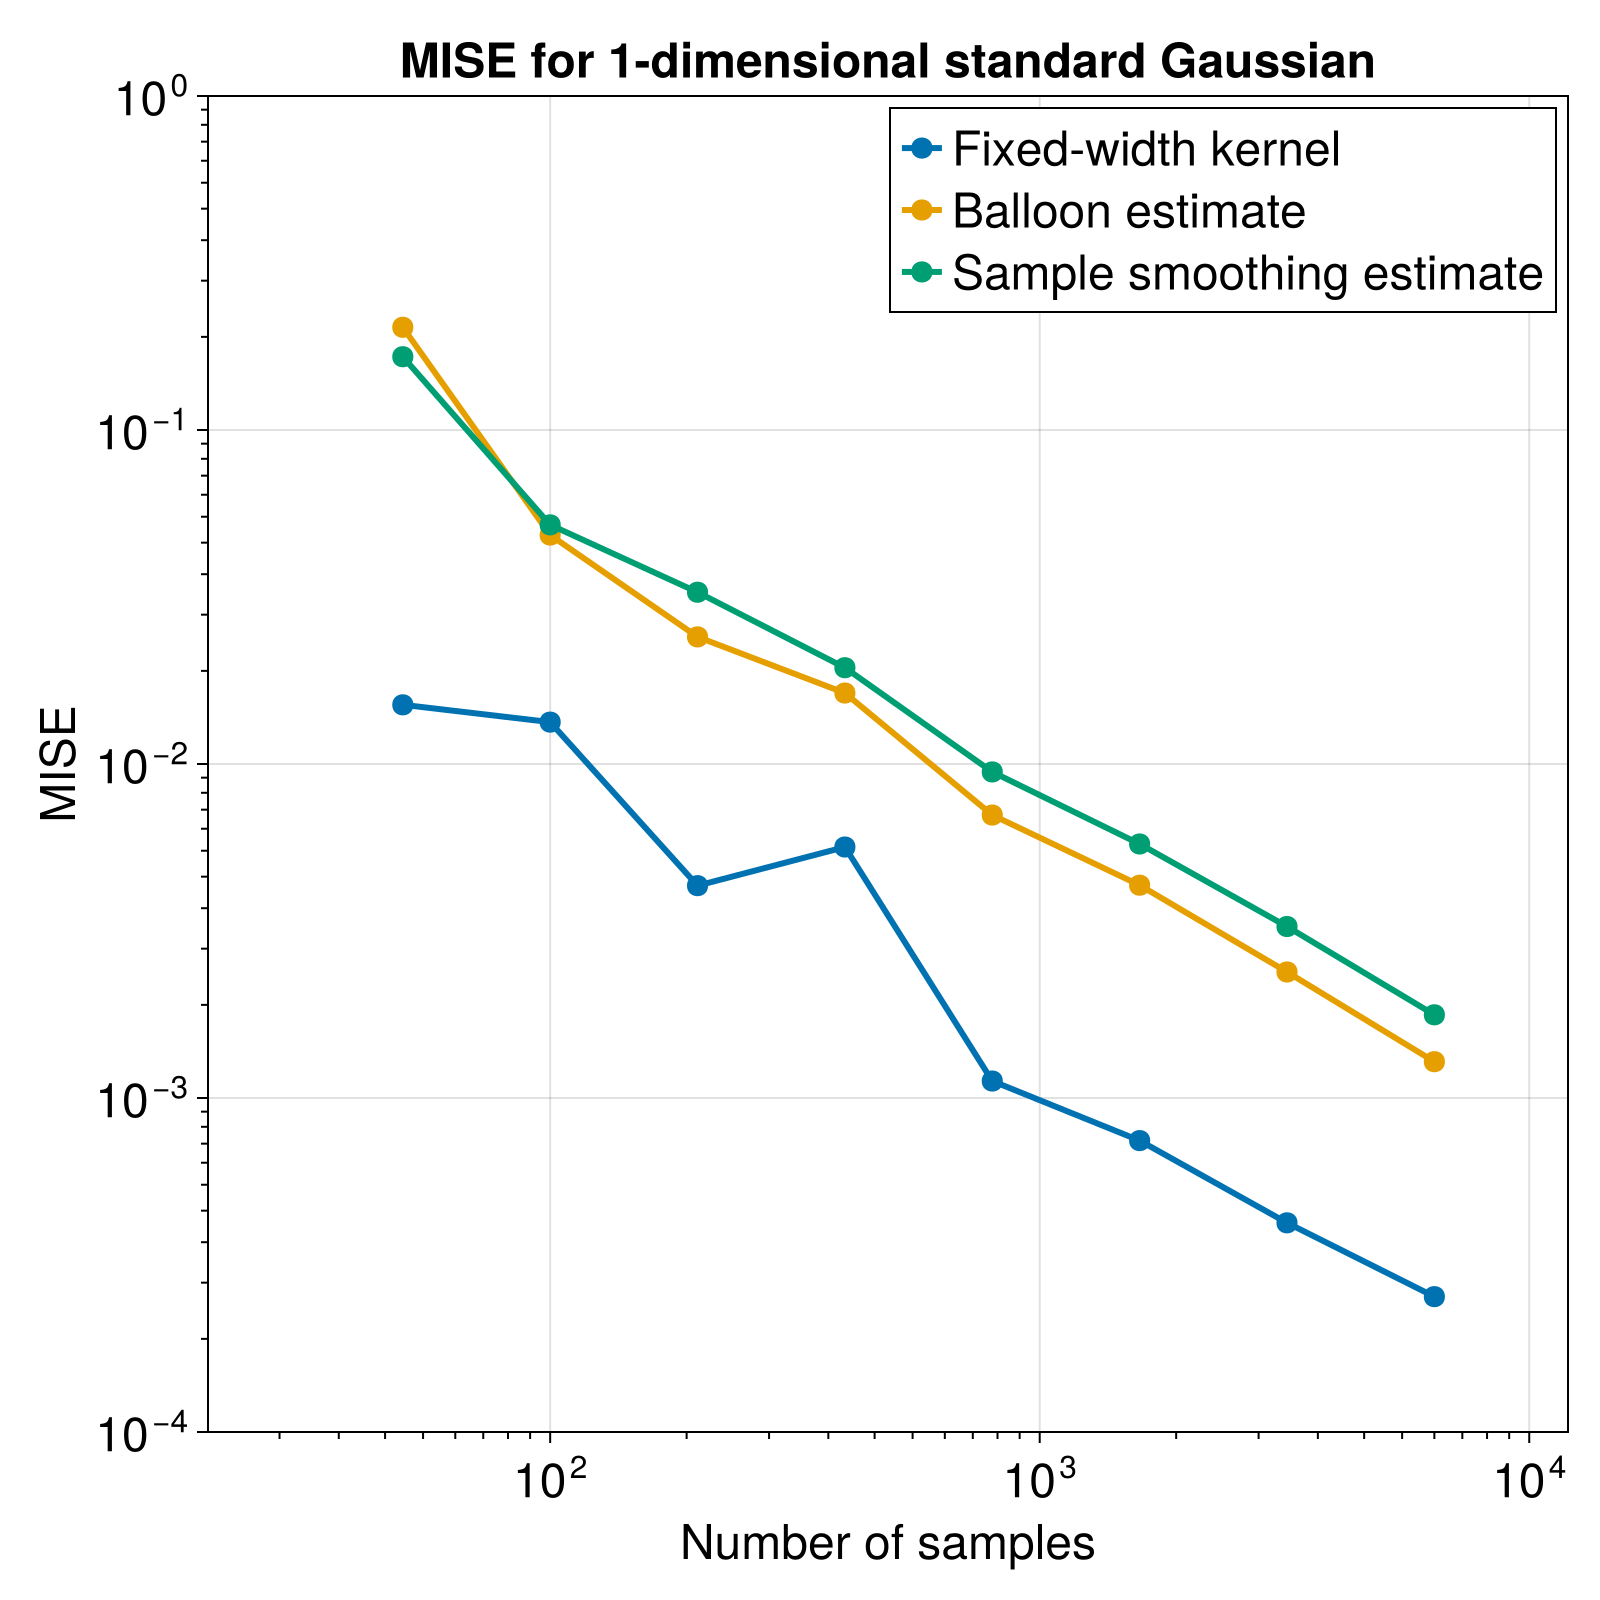
\includegraphics[width=.8\linewidth]{images/MISE_d=1.png}
  \caption{d=4}
  \label{fig:sfig2}
\end{subfigure}
\begin{subfigure}{.5\textwidth}
  \centering
  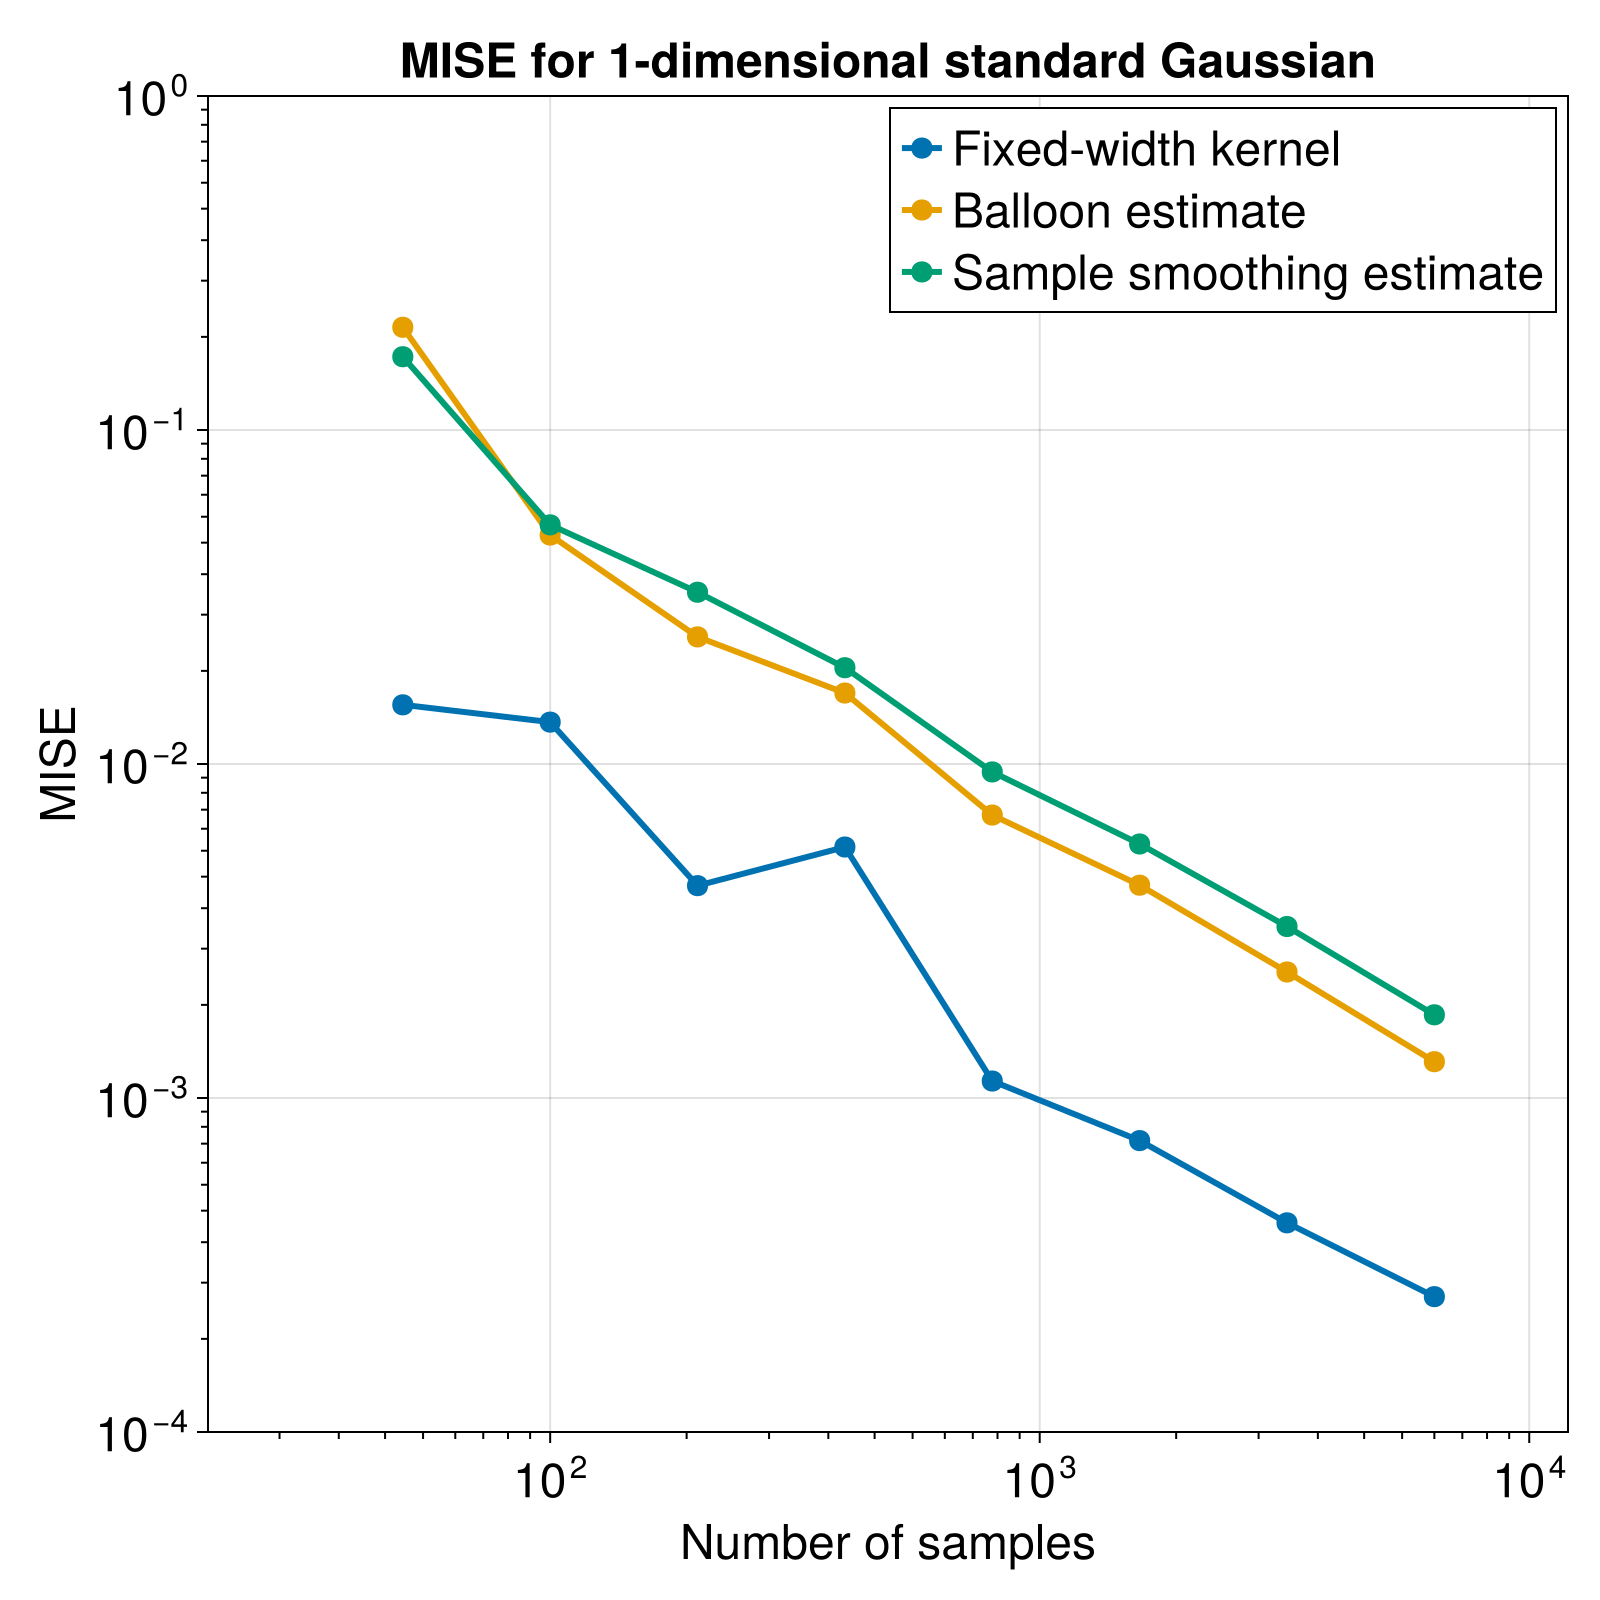
\includegraphics[width=.8\linewidth]{images/MISE_d=1.png}
  \caption{d=5}
  \label{fig:sfig1}
\end{subfigure}%
\begin{subfigure}{.5\textwidth}
  \centering
  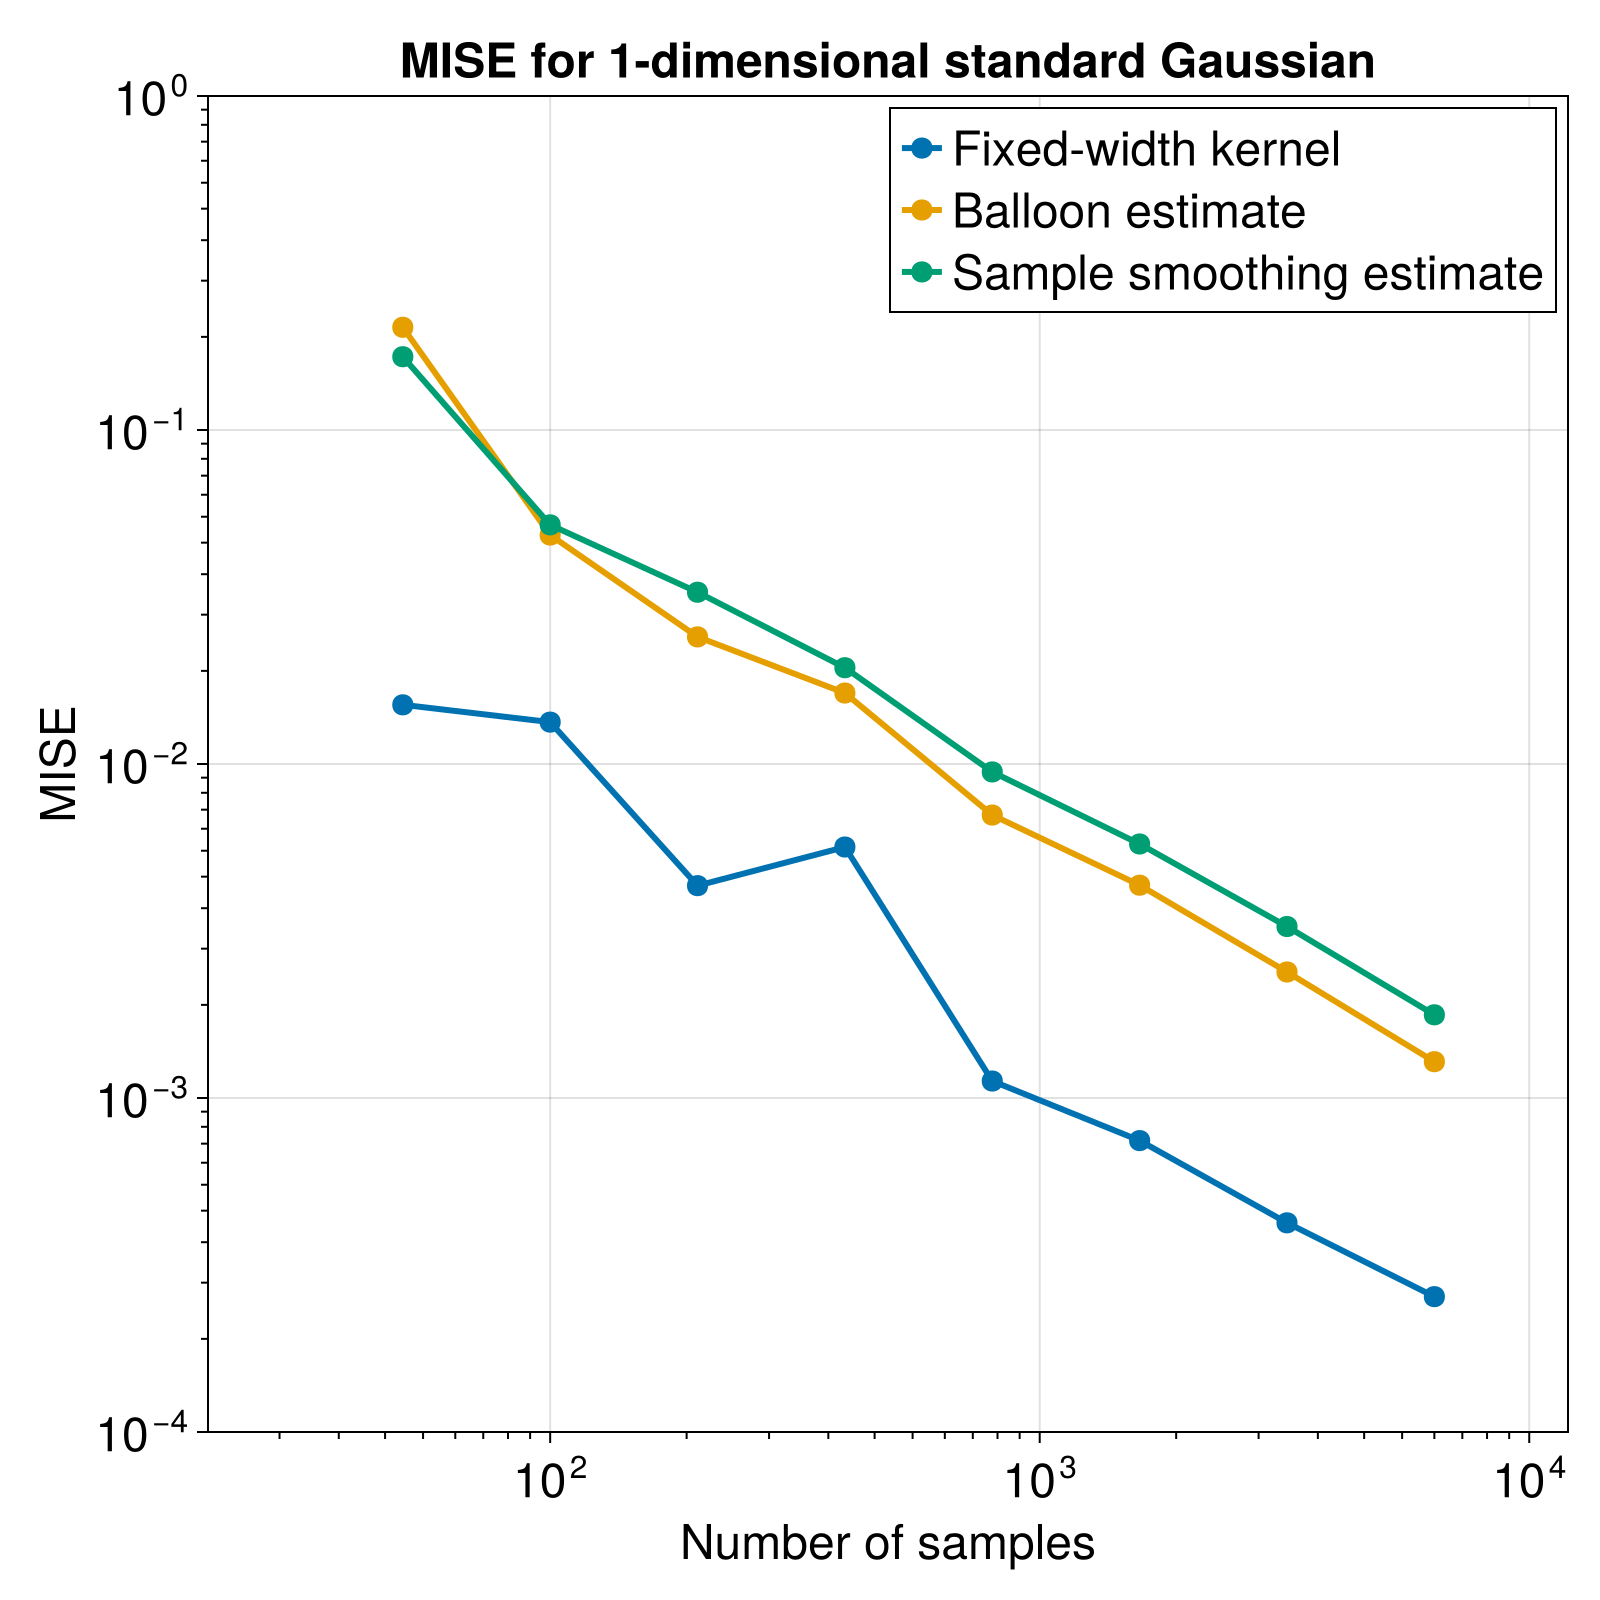
\includegraphics[width=.8\linewidth]{images/MISE_d=1.png}
  \caption{d=6}
  \label{fig:sfig2}
\end{subfigure}
\end{figure}

\section{Conclusion}

\printbibliography

\end{document}
